\documentclass{article}

\usepackage{tikz}
\usetikzlibrary{math}

\usepackage{xcolor}
\usepackage{tol_colors}

\let\oldcolor\color

\newcommand\normalvision{%
    \protect\renewcommand\color[1]{\oldcolor{##1}}%
}

\newcommand\protanopia{%
    \protect\renewcommand\color[1]{%
        \extractcolorspecs{##1}{\modelspec}{\colorspec}%
        \tikzmath{
            \r = array({\colorspec},0);
            \g = array({\colorspec},1);
            \b = array({\colorspec},2);
            \rp = pow(0.06425 + 0.677*pow(\g, 2.2) + 0.2802*pow(\r, 2.2), 1./2.2);
            \gp = pow(0.06425 + 0.677*pow(\g, 2.2) + 0.2802*pow(\r, 2.2), 1./2.2);
            \bp = pow(0.06425 + 0.95724*pow(\b, 2.2) + 0.02138*pow(\g, 2.2) - 0.02138*pow(\r, 2.2), 1./2.2);
        }%
        \oldcolor[rgb]{\rp,\gp,\bp}%
    }%
}

\newcommand\deuteranopia{%
    \protect\renewcommand\color[1]{%
        \extractcolorspecs{##1}{\modelspec}{\colorspec}%
        \tikzmath{
            \r = array({\colorspec},0);
            \g = array({\colorspec},1);
            \b = array({\colorspec},2);
            \rp = pow(0.01194 + 0.8806*pow(\g, 2.2) + 0.1115*pow(\r, 2.2), 1./2.2);
            \gp = pow(0.01194 + 0.8806*pow(\g, 2.2) + 0.1115*pow(\r, 2.2), 1./2.2);
            \bp = pow(0.01194 + 0.992052*pow(\b, 2.2) - 0.003974*pow(\g, 2.2) + 0.003974*pow(\r, 2.2), 1./2.2);
        }%
        \oldcolor[rgb]{\rp,\gp,\bp}%
    }%
}

\title{Easy colorblind-safe typesetting:\\ the \textbf{colorblind} package}
\author{Simon Pfahler}
\date{\today}

\begin{document}

\maketitle

\begin{figure}[ht]
    \centering
    \begin{tikzpicture}
        \newcommand{\dx}{1}
        \newcommand{\dy}{-1.5}
        \newcommand{\radius}{0.7}

        % test for non rgb color models
        \definecolor{hsbtest1}{rgb}{0.266, 0.465, 0.664}
        \definecolor{hsbtest2}{hsb}{0.266, 0.468, 0.664}
        
        % Tol's bright qualitative color scheme
        \fill[Tblue] (0,0) circle (\radius);
        \fill[Tcyan] (\dx,0) circle (\radius);
        \fill[Tgreen] (2*\dx,0) circle (\radius);
        \fill[Tyellow] (3*\dx,0) circle (\radius);
        \fill[Tred] (4*\dx,0) circle (\radius);
        \fill[Tpurple] (5*\dx,0) circle (\radius);
        \fill[Tgrey] (6*\dx,0) circle (\radius);

        \fill[hsbtest1] (8*\dx,0) circle (\radius);
        \fill[hsbtest2] (9*\dx,0) circle (\radius);
        
        {
        \protanopia
        \fill[Tblue, rounded corners=0.7*\radius cm]
            (0-\radius,\dy-0.7*\radius) rectangle ++(2*\radius, 1.4*\radius);
        \fill[Tcyan, rounded corners=0.7*\radius cm]
            (\dx-\radius,\dy-0.7*\radius) rectangle ++(2*\radius, 1.4*\radius);
        \fill[Tgreen, rounded corners=0.7*\radius cm]
            (2*\dx-\radius,\dy-0.7*\radius) rectangle ++(2*\radius, 1.4*\radius);
        \fill[Tyellow, rounded corners=0.7*\radius cm]
            (3*\dx-\radius,\dy-0.7*\radius) rectangle ++(2*\radius, 1.4*\radius);
        \fill[Tred, rounded corners=0.7*\radius cm]
            (4*\dx-\radius,\dy-0.7*\radius) rectangle ++(2*\radius, 1.4*\radius);
        \fill[Tpurple, rounded corners=0.7*\radius cm]
            (5*\dx-\radius,\dy-0.7*\radius) rectangle ++(2*\radius, 1.4*\radius);
        \fill[Tgrey, rounded corners=0.7*\radius cm]
            (6*\dx-\radius,\dy-0.7*\radius) rectangle ++(2*\radius, 1.4*\radius);

        \fill[hsbtest1, rounded corners=0.7*\radius cm]
            (8*\dx-\radius,\dy-0.7*\radius) rectangle ++(2*\radius, 1.4*\radius);
        \fill[hsbtest2, rounded corners=0.7*\radius cm]
            (9*\dx-\radius,\dy-0.7*\radius) rectangle ++(2*\radius, 1.4*\radius);

        }
        
        {
        \deuteranopia
        \fill[Tblue, rounded corners=0.7*\radius cm]
            (0-\radius,1.8*\dy-0.7*\radius) rectangle ++(2*\radius, 1.4*\radius);
        \fill[Tcyan, rounded corners=0.7*\radius cm]
            (\dx-\radius,1.8*\dy-0.7*\radius) rectangle ++(2*\radius, 1.4*\radius);
        \fill[Tgreen, rounded corners=0.7*\radius cm]
            (2*\dx-\radius,1.8*\dy-0.7*\radius) rectangle ++(2*\radius, 1.4*\radius);
        \fill[Tyellow, rounded corners=0.7*\radius cm]
            (3*\dx-\radius,1.8*\dy-0.7*\radius) rectangle ++(2*\radius, 1.4*\radius);
        \fill[Tred, rounded corners=0.7*\radius cm]
            (4*\dx-\radius,1.8*\dy-0.7*\radius) rectangle ++(2*\radius, 1.4*\radius);
        \fill[Tpurple, rounded corners=0.7*\radius cm]
            (5*\dx-\radius,1.8*\dy-0.7*\radius) rectangle ++(2*\radius, 1.4*\radius);
        \fill[Tgrey, rounded corners=0.7*\radius cm]
            (6*\dx-\radius,1.8*\dy-0.7*\radius) rectangle ++(2*\radius, 1.4*\radius);
        
        \fill[hsbtest1, rounded corners=0.7*\radius cm]
            (8*\dx-\radius,1.8*\dy-0.7*\radius) rectangle ++(2*\radius, 1.4*\radius);
        \fill[hsbtest2, rounded corners=0.7*\radius cm]
            (9*\dx-\radius,1.8*\dy-0.7*\radius) rectangle ++(2*\radius, 1.4*\radius);
        }
    \end{tikzpicture}
    \caption{Paul Tol's bright qualitative color scheme, normal vision, protanopia and deuteranopia}
\end{figure}

\begin{figure}[ht]
    \centering
    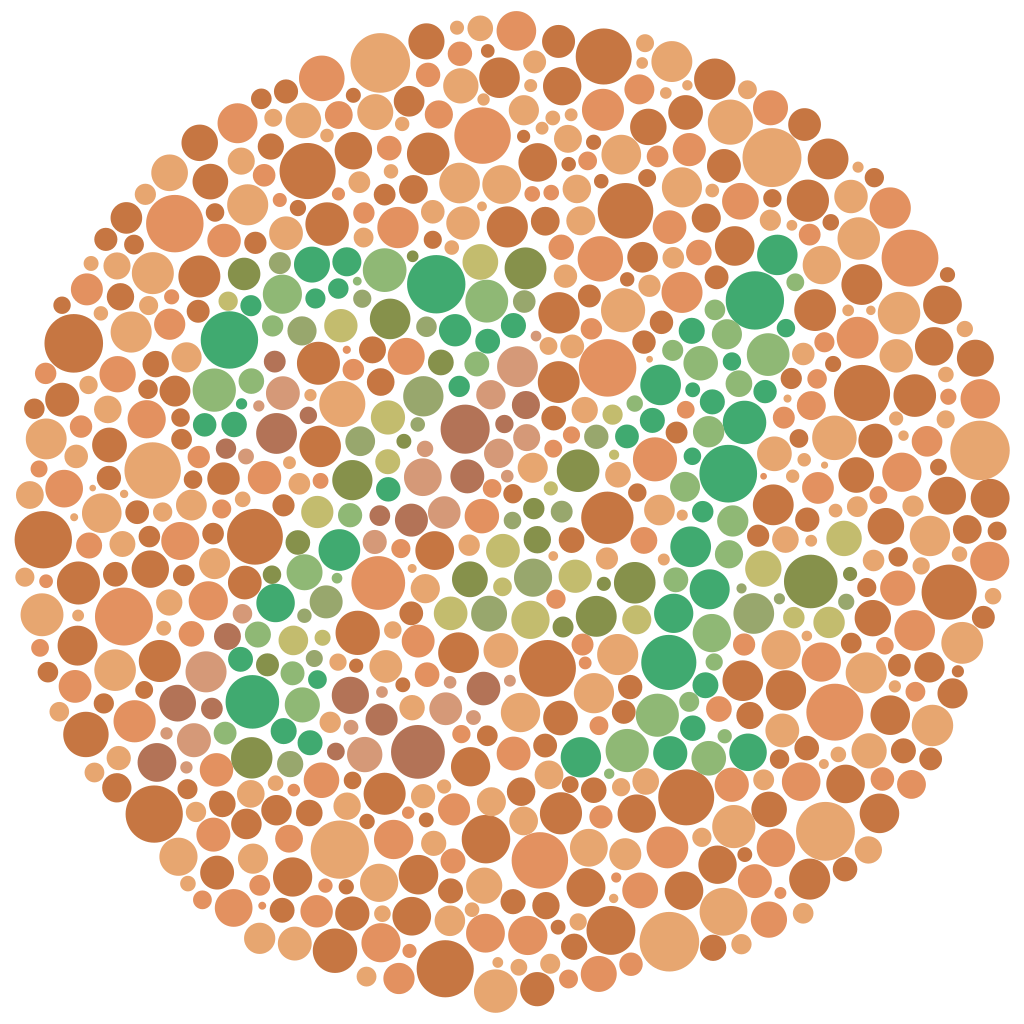
\includegraphics[width=0.3\textwidth]{Ishihara_9.png}
    \hspace{1cm}
    {\selectcolormodel{gray}
        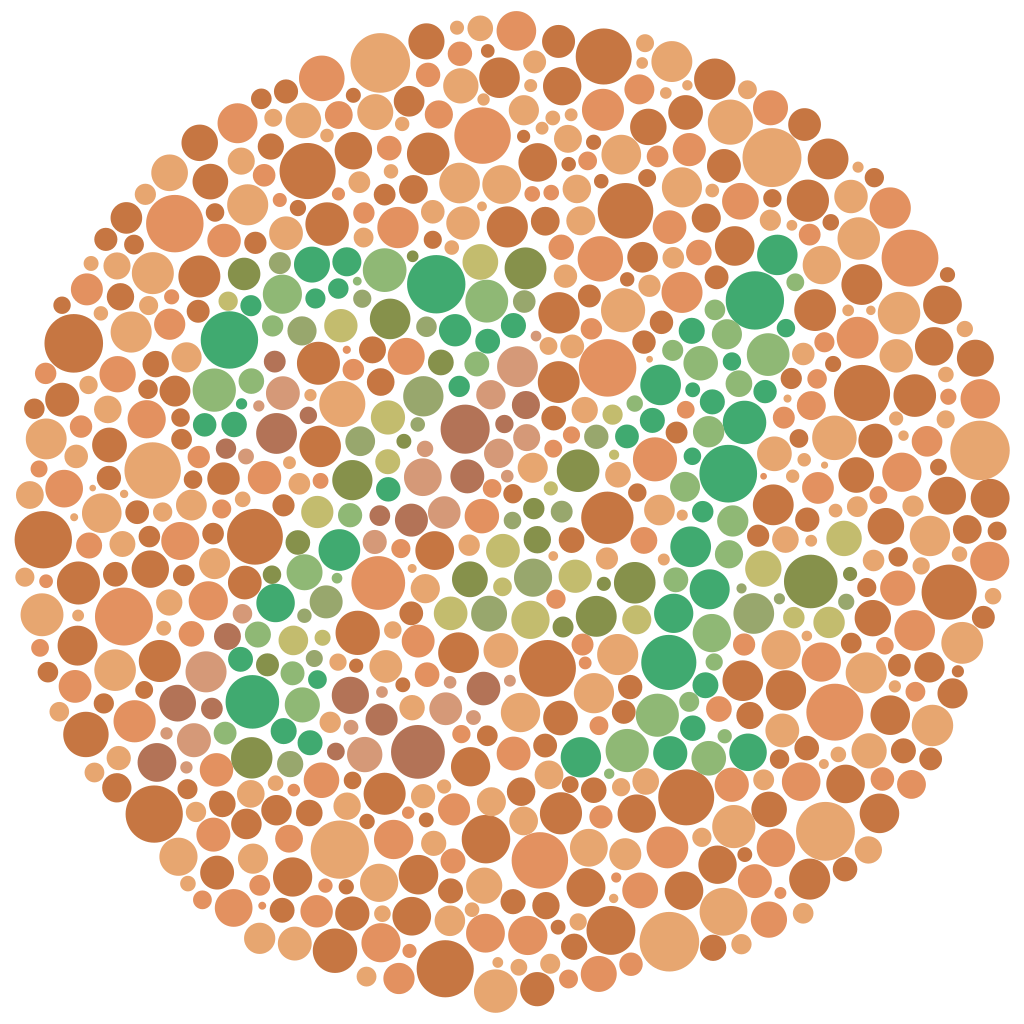
\includegraphics[decodearray={0 0 0 1 0 1}, width=0.3\textwidth]{Ishihara_9.png}
    }
    \caption{Ishihara colorblindness test, normal vision and without the {\color{red}red} channel}
\end{figure}

\end{document}
